\RequirePackage[l2tabu,orthodox]{nag}

% TODO: decide if one-sided/two-sided or whatever

\documentclass[headsepline,footsepline,footinclude=false,fontsize=11pt,paper=a4,listof=totoc,bibliography=totoc,BCOR=12mm,DIV=20]{scrbook} % two-sided

% \documentclass[headsepline,footsepline,footinclude=false,oneside,fontsize=11pt,paper=a4,listof=totoc,bibliography=totoc]{scrbook} % one-sided

\PassOptionsToPackage{table,svgnames,dvipsnames}{xcolor}

\usepackage[utf8]{inputenc}
\usepackage[T1]{fontenc}
\usepackage[sc]{mathpazo}
\usepackage[ngerman]{babel}
\usepackage{upgreek}
\usepackage[autostyle]{csquotes}
\usepackage{siunitx} %SI-units will not be set in italics using this package

%Blindtext - kann entfernt werden
\usepackage{blindtext}

%defining bibliography&citation
\usepackage[
  backend=biber,
  url=false,
  style=authoryear,
  maxbibnames=99,
  maxcitenames=1,
  firstinits=true,
  doi=false,
  isbn=false,
  sorting=nyt,
  uniquename=init]{biblatex} % TODO: BIBLIOGRAPHYSETTINGS
\DefineBibliographyStrings{ngerman}{andothers={et\ al\adddot}} % "u.a." zu "et al." 
\DefineBibliographyStrings{ngerman}{and={\&}} % "und" zu "&"

\usepackage{graphicx}
\usepackage{lstautogobble}
\usepackage{booktabs}
\usepackage{scrhack}
\usepackage[final]{microtype}
\usepackage{caption}
\usepackage[hidelinks]{hyperref} % hidelinks removes colored boxes around references and links
\usepackage[toc,nonumberlist,acronym]{glossaries}
\bibliography{bibliography/library}
\setkomafont{disposition}{\normalfont\bfseries} % use serif font for headings
\linespread{1.05} % adjust line spread for mathpazo font

% Settings for glossaries
\renewcommand{\glsnamefont}[1]{\normalfont\bfseries #1} % use serif font for glossary entry titles
\makeglossaries{}

% Basic information for cover & title page
\newcommand*{\getUniversity}{Technische Universität München}
\newcommand*{\getFaculty}{Fakultät für Medizin}
\newcommand*{\getTitle}{Oligomerization of $\upbeta_2$-Adrenergic Receptors}
\newcommand*{\getTitleGer}{Oligomerisierung von $\upbeta_2$-Adrenorezeptoren}
\newcommand*{\getAuthor}{Stephan Skawran}
\newcommand*{\getDoctype}{Dissertation zur Erlangung des akademischen Titels Dr. med.}
\newcommand*{\getSupervisor}{Prof. Dr. Dr. Stefan Engelhardt}
\newcommand*{\getAdvisor}{Dr. Andrea Ahles}
\newcommand*{\getSubmissionDate}{TODO: Submission date}
\newcommand*{\getSubmissionLocation}{München}


\begin{document}

\begin{titlepage}
  % HACK for two-sided documents: ignore binding correction for cover page.
  % Adapted from Markus Kohm's KOMA-Script titlepage=firstiscover handling.
  % See http://mirrors.ctan.org/macros/latex/contrib/koma-script/scrkernel-title.dtx,
  % \maketitle macro.
  \oddsidemargin=\evensidemargin\relax
  \textwidth=\dimexpr\paperwidth-2\evensidemargin-2in\relax
  \hsize=\textwidth\relax

  \centering

  \vspace{40mm}
  
\includegraphics[width=40mm]{logos/tum}

  \vspace{5mm}
  {\huge\MakeUppercase{\getFaculty{}}}\\

  \vspace{5mm}
  {\large\MakeUppercase{\getUniversity{}}}\\

  \vspace{20mm}
  {\Large \getDoctype{}}

  \vspace{15mm}
  {\huge\bfseries \getTitle{}}

  \vspace{15mm}
  {\LARGE \getAuthor{}}

  \vspace{20mm}
  
\includegraphics[width=20mm]{logos/faculty}
\end{titlepage}


\frontmatter{}

\begin{titlepage}
{\par \centering

  \vspace{40mm}
  
\includegraphics[width=40mm]{logos/tum}

  \vspace{5mm}
  {\huge\MakeUppercase{\getFaculty{}}}\\
    
  \vspace{5mm}
  {\large\MakeUppercase{\getInstitute{}}}\\

  
\par}

  \vspace{20mm}
  \large{\noindent Vollständiger Abdruck der von der Fakultät für Medizin der Technischen Universität München zur Erlangung des akademischen Grades eines Dr. med. genehmigten Dissertation.}

  \vspace{20mm}
{\par \centering
  {\huge\bfseries \getTitleGer{}}\\
  \vspace{5mm}
  {\LARGE \getAuthor{}}
  \vspace{15mm}
  
  \begin{tabular}{l l}
    \large{Vorsitzender:}                    & \large{\getSupervisor{}} \\
    \large{Prüfer der Dissertation:}        & \large{1.} \\
                                    & \large{2.} \\
                                    & \large{3.} \\
    \end{tabular}
\\
\par}

\vspace {15mm}

\large{\noindent Die Dissertation wurde am \getSubmissionDate{} bei der Technischen Universität München eingereicht und durch die Fakultät für Medizin am \getSubmissionDate{} angenommen}. 

\vspace {20mm}
  \centering
  
\includegraphics[width=20mm]{logos/faculty}
\end{titlepage}

\thispagestyle{empty}
\vspace*{0.8\textheight}
\noindent
Ich erkläre an Eides statt, dass ich diese, bei der Fakultät für Medizin der TUM zur Promotionsprüfung vorgelegte Arbeit ohne sonstige Hilfe erstellt und bei der Abfassung nur die gemäß § 6 Abs. 6 und 7 Satz 2 angegebenen Hilfsmittel benutzt habe.
\vspace{15mm}
\noindent
\getSubmissionLocation{}, \getSubmissionDate{} \hspace{5cm} \getAuthor{}

\cleardoublepage{}

\addcontentsline{toc}{chapter}{Danksagung}
\thispagestyle{empty}

\vspace*{2cm}

\begin{center}
{\usekomafont{section} Danksagung}
\end{center}

\vspace{1cm}

Besonders möchte ich Prof. Dr. Dr. Engelhardt, dem Leiter des Instituts für Pharmakologie und Toxikologie der Technischen Universität München für die Möglichkeit danken, meine Dissertation unter seiner Leitung durchführen zu dürfen. 

\vspace{2cm}

Besonderer Dank gilt Dr. Andrea Ahles für ihre stete Diskussionsbereitschaft und Anregungen, die maßgeblich zum Gelingen dieser Arbeit beigetragen haben.

\vspace{2cm}

Für die optimistische und immer hilfsbereite Arbeitsatmosphäre des gesamten Laborteams möchte ich mich vielmals bedanken.  

%\cleardoublepage{}

\glsaddall{} % add all defined terms to glossary, even if not referenced in text
%{name}{Abkürzung}{Langform}
\newacronym{zb}{zB}{zum Beispiel}
\newacronym{cd}{CD}{Compact Disk}
\newacronym{aa}{aA}{am Arsch}

\printglossary[title=Verzeichnis der Abkürzungen,type=\acronymtype]

\microtypesetup{protrusion=false}
\tableofcontents{}
\microtypesetup{protrusion=true}

\mainmatter{}

\chapter{Introduction}\label{chapter:introduction}

\section{Firstsection}
Citation test~\parencite{latex}.

\subsection{Subsection}
See~\autoref{fig:sample}.

\begin{figure}[htsb]
  \centering
  
\includegraphics{logos/tum}
  \caption[Example figure]{An example for a figure.}\label{fig:sample}
\end{figure}

\section{Section}

See~\autoref{tab:sample}, \autoref{fig:sample-drawing}, \autoref{fig:sample-plot}, \autoref{fig:sample-listing}.

\begin{table}[htsb]
  \caption[Example table]{An example for a simple table.}\label{tab:sample}
  \centering
  \begin{tabular}{l l l l}
    \toprule
      A & B & C & D \\
    \midrule
      1 & 2 & 1 & 2 \\
      2 & 3 & 2 & 3 \\
    \bottomrule
  \end{tabular}
\end{table}

\begin{figure}[htsb]
  \centering
  % This should probably go into a file in figures/
  \begin{tikzpicture}[node distance=3cm]
    \node (R0) {$R_1$};
    \node (R1) [right of=R0] {$R_2$};
    \node (R2) [below of=R1] {$R_4$};
    \node (R3) [below of=R0] {$R_3$};
    \node (R4) [right of=R1] {$R_5$};

    \path[every node]
      (R0) edge (R1)
      (R0) edge (R3)
      (R3) edge (R2)
      (R2) edge (R1)
      (R1) edge (R4);
  \end{tikzpicture}
  \caption[Example drawing]{An example for a simple drawing.}\label{fig:sample-drawing}
\end{figure}

\begin{figure}[htsb]
  \centering

  \pgfplotstableset{col sep=&, row sep=\\}
  % This should probably go into a file in data/
  \pgfplotstableread{
    a & b    \\
    1 & 1000 \\
    2 & 1500 \\
    3 & 1600 \\
  }\exampleA
  \pgfplotstableread{
    a & b    \\
    1 & 1200 \\
    2 & 800 \\
    3 & 1400 \\
  }\exampleB
  % This should probably go into a file in figures/
  \begin{tikzpicture}
    \begin{axis}[
        ymin=0,
        legend style={legend pos=south east},
        grid,
        thick,
        ylabel=Y,
        xlabel=X
      ]
      \addplot table[x=a, y=b]{\exampleA};
      \addlegendentry{Example A};
      \addplot table[x=a, y=b]{\exampleB};
      \addlegendentry{Example B};
    \end{axis}
  \end{tikzpicture}
  \caption[Example plot]{An example for a simple plot.}\label{fig:sample-plot}
\end{figure}

\begin{figure}[htsb]
  \centering
  \begin{tabular}{c}
  \begin{lstlisting}[language=SQL]
    SELECT * FROM tbl WHERE tbl.str = "str"
  \end{lstlisting}
  \end{tabular}
  \caption[Example listing]{An example for a source code listing.}\label{fig:sample-listing}
\end{figure}
 %Beispielseiten

\chapter{Einleitung}\label{chapter:einleitung}

\section{G-Protein-gekoppelte Rezeptoren (GPCR)}

\section{$\beta$-adrenerge Rezeptoren}
\subsection{Das $\beta$-adrenerge System}
\subsection{Polymorphismen der $\beta$-adrenergen Rezeptoren}
\subsection{Rezeptorinternalisierung}


\section{Oligomerisierung G-Protein-gekoppelter Rezeptoren}
\subsection{Homo- und Heterooligomerisierung G-Protein-gekoppelter Rezeptoren}
\subsection{Pharmakologische Anwendung}

\section{Methoden zur Untersuchung der Oligomerisierung von Rezeptoren}
\subsection{time-resolved FRET}

\section{Zielsetzung dieser Arbeit}
\chapter{Material \& Methoden}\label{chapter:materialmethoden}

\section{Plasmide}
Die folgenden Plasmide stammen entweder aus dem Laborbestand oder wurden von NEB GmbH (Frankfurt a. M.) erworben. Sie wurden unverändert transfiziert.

\begin{table}[htsb]
  \begin{tabular}{l l l l}
    \toprule
      A & B & C & D \\
    \midrule
      1 & 2 & 1 & 2 \\
      2 & 3 & 2 & 3 \\
    \bottomrule
  \end{tabular}
\end{table}

In den angegebenen Vektor wurden folgende Inserts kloniert. Dazu wurde die Methode der homologen Rekombination als Teil der Gateway-Technologie (Invitrogen, Karlsruhe) verwendet.

\begin{table}[htsb]
    \begin{tabular}{lll}
        \toprule
        Vector		&	Insert		& 	Reference	\\
        \midrule
        pSNAPf		&				&	New England Biolabs GmbH (Frankfurt a. M.)\\
        pCLIPf		&				&	New England Biolabs GmbH (Frankfurt a. M.)\\
        pSNAPf		&	ADRB2-16Gly	&	New England Biolabs GmbH (Frankfurt a. M.)\\
        pDONR221	&	ADRB2-16Arg	    &	IPT (TU München)\\
    \bottomrule
    \end{tabular}
\end{table}

In den angegebenen Vektor wurden folgende Inserts kloniert. Dazu wurde die Methode der homologen Rekombination als Teil der Gateway-Technologie (Invitrogen, Karlsruhe) verwendet.

\begin{table}[htsb]
\begin{tabular}{lll}
\toprule
Vektor		&	Insert		&	Polymorphismus / Mutation\\
\midrule
pSNAPf		&	5mis-ADRB2	&	Arg16, Tyr284\\
pSNAPf		&	ADRB2		&	Arg16\\
pCLIPf		&	ADRB2		&	Arg16\\
\bottomrule
\end{tabular}
\end{table}

\section{Bakterien}

\begin{tabular}{ll}
\toprule
Name		    &	Referenz\\
\midrule
E. coli (DH10B)	&    IPT (TU München)\\
\bottomrule
\end {tabular}


\section{Zelllinien}
text\\

\begin{tabular}{lll}
\toprule
Name		&	Source (Organ)				&	Reference\\
\midrule
HEK293		&	Human Embryonic Kidney		&	IPT (TU München)\\
HeLa		&	Human Cervix Epithelium		&	IPT (TU München)\\
\bottomrule
\end {tabular}\\

Based on the specified cell lines, the following stably expressing cell lines were generated:\\

\begin{tabular}{lll}
\toprule
Name		&	Stably Overexpressed Protein	&	Polymorphic Variants\\
\midrule
HEK293		&	$\beta_2$-adrenoreceptor		&	Arg16, Gly16, Tyr284\\
HeLa		&	$\beta_2$-adrenoreceptor		&	Arg16, Gly16, Tyr284\\
\bottomrule
\end{tabular}

\section{Chemicals \& Reagents}
If not specified otherwise, all chemicals and reagents were obtained from Applichem (Darmstadt), Carl Roth (Karlsruhe), Merck (Darmstadt) and Sigma-Aldrich (Taufkirchen). \\

\begin{tabular}{lll}
\toprule
Name							&	Company\\
\midrule
BG-Alexa488						&	New England Biolabs GmbH (Frankfurt a. M.)\\
BG-d2							&	Cisbio Bioassys (Codolet, France)\\
BG-Terbium						&	Cisbio Bioassys (Codolet, France)\\
\bottomrule
\end {tabular}

\section{Enzyme}

\begin{tabular}{lll}
\toprule
Name							&	Company\\
\midrule
DNA Ligase T4						&	New England Biolabs (Frankfurt a. M.)\\
DNA Polymerase AccuPrime \textit{Pfx}	&	Invitrogen (Karlsruhe)\\
DNA Polymerase Quikchange Lightning	&	Agilent Technologies (Waldbronn)\\
Restriction Endonucleases			&	New England Biolabs (Frankfurt a. M.)\\
Restriction Enzyme DpnI				&	Agilent Technologies (Waldbronn)\\
\bottomrule
		
\end {tabular}


\section{Oligonukleotidprimer}

\begin{tabular}{lll}
\toprule
Name		&	Sequenz 					&	Produkt\\
\midrule
ADRB2-SbfI-for	&&\\
ADRB2-XhoI-rev	&	AAA AAA CCT GCA GGC GGG CAA CCC GGG AAC GG	&	\textit{SbfI}-\textbf{ADRB2}-\textit{XhoI}\\
ADRB2-c850t\_t851a\_for	& 	CAT GGG CAC TTT CAC CTA CTG CTG GCT GCC CTT C & ADRB2(Tyr284)\\
ADRB2-c850t\_t851a\_rev	&	GAA GGG CAG CCA GCA GTA GGT GAA AGT GCC CAT G &\\
\bottomrule
\end{tabular}

\section{Pharmaka}
\begin{tabular}{lll}
\toprule
Name			&	Type										&	Company\\
\midrule
Alprenolol		&	$\beta_2$\-Adrenorezeptoragonist				&	Sigma-Aldrich GmbH\\
ICI-118,551		&	$\beta_2$\-inverser Adrenorezeptoragonist		&	Sigma-Aldrich GmbH\\
Isoproterenol	&	$\beta_2$\-Adrenorezeptoragonist				&	Sigma-Aldrich GmbH\\
Epinephrine		&	natürlihcer Adrenorezeptoragonist			& 	Sigma-Aldrich GmbH\\
\bottomrule

\end{tabular}
\chapter{Ergebnisse} \label{chapter:ergebnisse}
\section{Generierung von $\beta_2$-Adrenorezeptoren mit dem SNAP-tag} \label{klonierung}
Zur Untersuchung der Oligomerisierung des \gls{beta2} wurde der Rezeptor so modifiziert, dass er über eine extrazelluläre Komponente verfügte, die Untersuchungen mit fluoreszierenden Substraten ermöglichte. Der SNAP-tag ermöglicht über seine O\textsuperscript{6}-Alkylguanin-DNA-Alkyltransferase-Aktivität die kovalente Bindung nahezu beliebiger Moleküle \parencite{Gronemeyer2006}. Die gewünschten Fluorophore müssen dazu eine O\textsuperscript{6}-Benzylguanin oder O\textsuperscript{6}-Alkylguanin-Gruppe tragen. Viele Fluorophore, darunter trFRET-kompatible, sind kommerziell verfügbar. Die Funktionsweise ist in Abbildung \ref{fig:snap-tag} dargestellt

\begin{figure}[htp]
    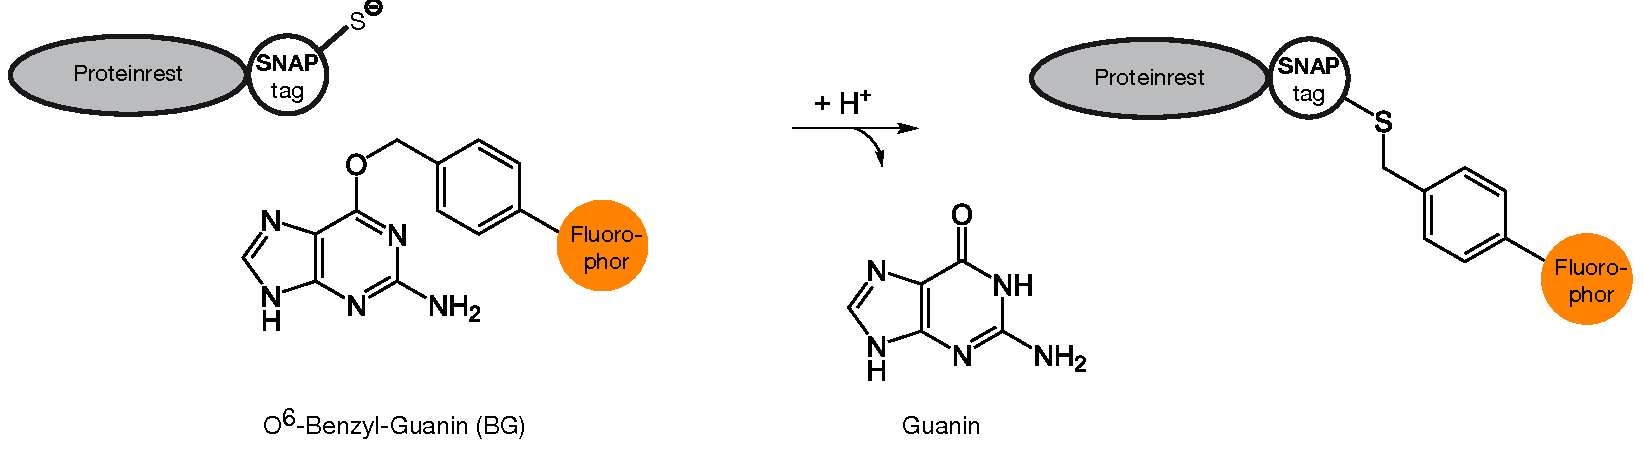
\includegraphics[width=0.97\textwidth]{SNAP-tag.pdf}
    \caption{\textbf{Funktionsweise des SNAP-tag}}
    \label{fig:snap-tag}
\end{figure}

Darauf basierend wurden Vektoren kloniert, die den \gls{beta2} trugen, der N-terminal über den SNAP-tag verfügte. 
\\ \\
Mittels Fluoreszenzmikroskopie konnte initial gezeigt werden, dass mit der N-terminalen Modifikation des \gls{beta2} keine Membranexpression des \gls{beta2} mehr erfolgte (s. Abb. \ref{fig:stainsnap} in \ref{snapmikro}). Infolgedessen wurde weiter N-terminal eine Proteinsequenz zur Membraninsertion verwendet, die zur zufriedenstellenden Expression des \gls{beta2} führte. 
\\ \\
In Abbildung \ref{fig:klonierung} sind schematisch die Klonierungsstrategien zu den final verwendeten Vektoren dargestellt. Es wurden Expressionsvektoren erzeugt, die die SNAP-getaggten natürlich vorkommenden Varianten Arg16 und Gly16 des \gls{beta2} exprimierten.
\\ \\ 
Darüber hinaus wurden zwei weitere Expressionssysteme generiert: Ein Vektor, der den \gls{beta2} mit dem SNAP-tag im zweiten extrazellulären Loop trug, sowie einen weiteren, der die in der Literatur als dimerisierungsdefizient beschriebene Variante Tyr284 \parencite{Salahpour2004} enthielt.
\\ \\
Für zukünftige Anwendung wurden außerdem analog Vektoren kloniert, die den mit dem CLIP-tag versehenen \gls{beta2} trugen (nicht dargestellt). 

\begin{figure}[htp]
    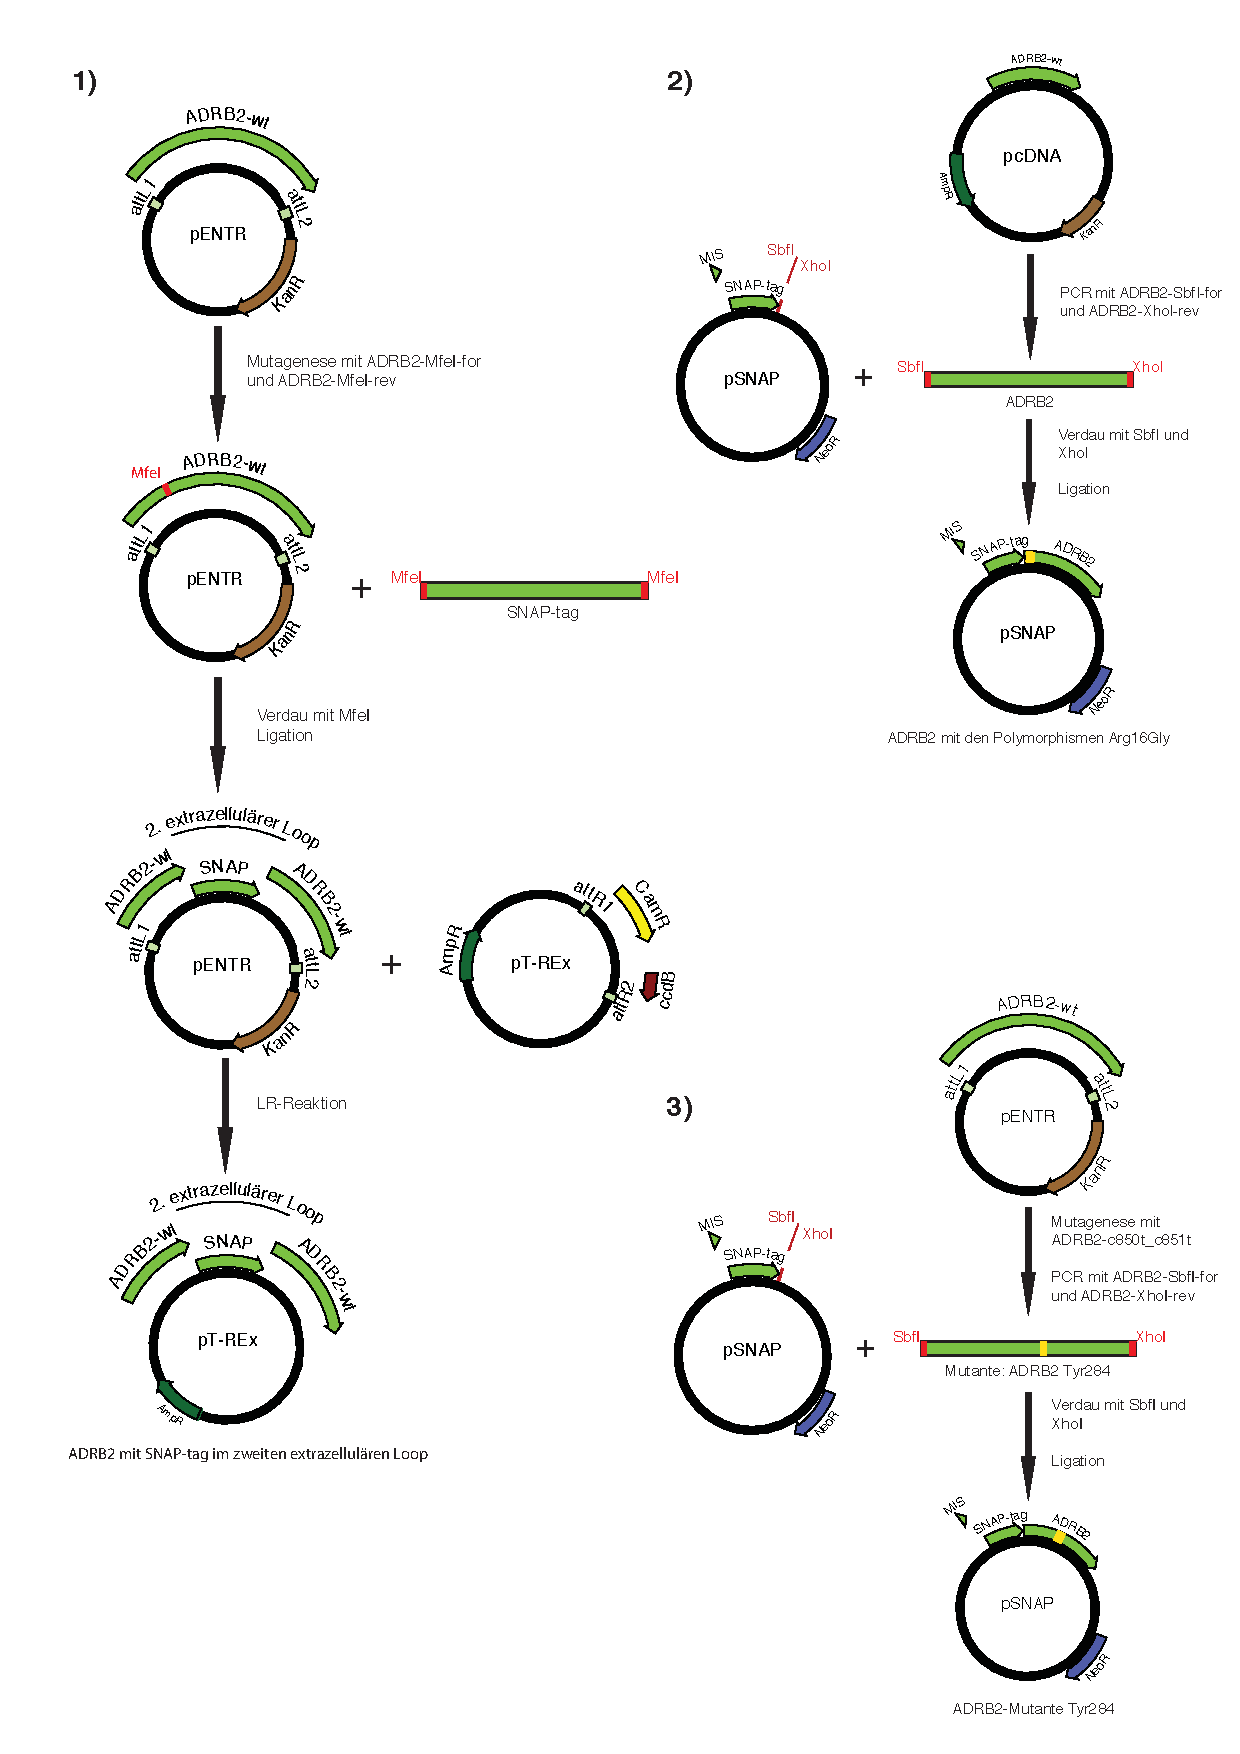
\includegraphics[width=0.97\textwidth]{cloning.pdf}
    \caption{\textbf{Klonierungsstrategien}: \textbf{1)} Generierung eines Expressionsvektors mit dem SNAP-tag im zweiten extrazellulären Loop des \gls{beta2}; \textbf{2)} SNAP-tag am N-Terminus des \gls{beta2}; \textbf{3)} SNAP-tag am N-Terminus der dimerisierungsdefizienten Mutante des \gls{beta2}}
    \label{fig:klonierung}
\end{figure}

\section{Fluoreszenzmikroskopie des \gls{beta2} mit dem SNAP-tag} \label{snapmikro}

Die Charakterisierung der Oligomerisierung des \gls{beta2} zunächst außer Acht gelassen, wurden zuerst Fluoreszenzfärbungen mit SNAP-Substraten durchgeführt. Dabei sollte geprüft werden, ob der mit dem SNAP-tag versehene Rezeptor korrekt in die Zellmembran integriert wird, bzw. noch trivialer, ob die Transfektion mit zufriedenstellender Effizienz gelungen war.

Wie in \ref{klonierung} beschrieben, konnten erfolgreich Vektoren erzeugt werden, die den mit dem SNAP-tag versehenen \gls{beta2} trugen. Diese Plasmide konnten in die HeLa- und HEK293-Zelllinien transient transfiziert werden.

\begin{figure}[htp]
    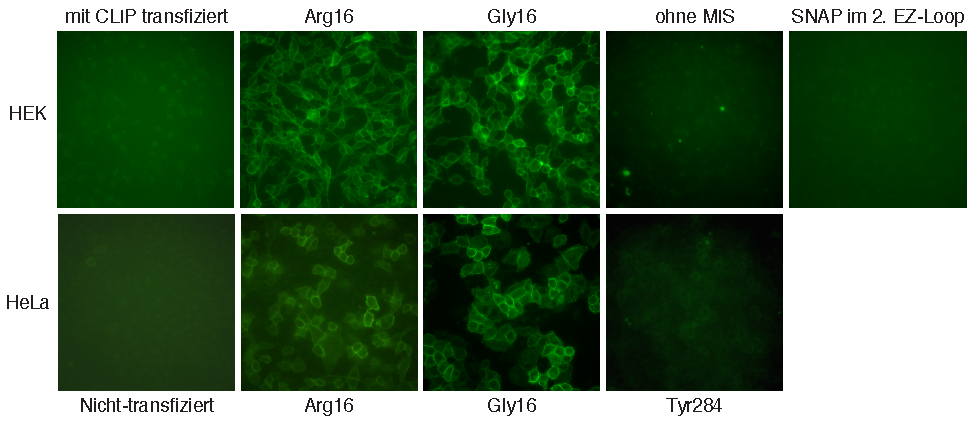
\includegraphics[width=1.0\textwidth]{snap_fluormikro.pdf}
    \caption{\textbf{Fluoreszenzfärbung mit SNAP-Substraten:} transient exprimierende HEK293- und stabile HeLa-Zellen.}
    \label{fig:stainsnap}
\end{figure}

Zunächst wurden direkt nach der Transfektion in HEK293-Zellen mit BG-Alexa-488 SNAP-basierte Fluoreszenzfärbungen durchgeführt. Dabei zeigten sich die in Abbildung \ref{fig:stainsnap} in der mit HEK gekennzeichneten Zeile dargestellten Expressionsmuster: Als Negativkontrolle dienten entweder nicht transfizierte Zellen oder Zellen, die mit dem \gls{beta2} transfiziert worden waren, der den CLIP-tag trug. Für den Arg16Gly-Polymorphismus zeigte sich in beiden Fällen ein deutliches Membranexpressionsmuster mit vernachlässigbarem Hintergrundsignal. Für die Variante des Vektors, der N-terminal vor dem SNAP-tag kein Membraninsertionssignal enthielt, war keine Membranfärbung nachweisbar. Auch die Variante des \gls{beta2}, die den SNAP-tag im zweiten extrazellulären Loop trug, war fluoreszenzmikroskopisch kein Membranexpressionsmuster erkennbar. Die Tyr284-Variante, wurde in HeLa-Zellen transfiziert. Dort war keine Membranfärbung erkennbar.
\\ \\
HEK293-Zellen eigneten sich aufgrund ihrer geringen Adhärenz nicht für die weiteren Versuchsreihen, die allesamt häufiges Waschen benötigten. Somit wurden stabile Zelllinien nur mit den stärker adhärenten HeLa-Zellen generiert. Diese zeigten in der Fluoreszenzmikroskopie eine den HEK293-Zellen vergleichbare Membranexpression. Die Ergebnisse sind in Abbildung \ref{fig:stainsnap} dargestellt. Sowohl bei der Arg16- als auch bei der Gly16-Variante des \gls{beta2} war eine klare lineare Membranfärbung feststellbar.

\section{Oligomerisierung des \gls{beta2} mit SNAP-tag}
Zur Analyse der Oligomerisierung des \gls{beta2} wurde der in der Einleitung beschriebene trFRET-Ansatz verwendet. Dazu wurden zuerst mit trFRET kompatible Fluorophore, die an Substrate des SNAP-tag gekoppelt waren, in unterschiedlichen Versuchsreihen zur Untersuchung der prinzipiellen Oligomerisierung des modifizierten \gls{beta2} eingesetzt. In den in Abschnitt \ref{ligandenfret} vorgestellten Ergebnissen konnten dann fluoreszierende Liganden des unveränderten \gls{beta2} in analogen Versuchsreihen die Oligomerisierung des Rezeptors zeigen.

\subsection{\gls{trfret} mit SNAP-Substraten}
Mit Hilfe der trFRET-Methode konnte die räumliche Interaktion von Molekülen es \gls{beta2} nachgewiesen werden. Dazu wurde in einem ersten Schritt die optimale Konzentration des Donorfluorophors bestimmt. Darauf konnte eine räumliche Interaktion gemessen werden. In einem letzten Schritt wurde gezeigt, dass diese spezifisch war.

\subsubsection{Bestimmung der Sättigungskinetik der SNAP-Substrate}
Zur optimalen Einstellung der Konzentrationen der verwendeten SNAP-Substrate wurden Sättigungsassays durchgeführt. Dazu wurden steigende Konzentrationen des mit dem Donorfluorophor Lumi4 verbundenen SNAP-Substrats (Lumi4-BG) mit Zellen inkubiert, die den SNAP-getaggten \gls{beta2} trugen. Diese Zellen waren zuvor fluoreszenzmikroskopisch auf ihre Expression untersucht worden. Als Negativkontrolle und zur Abschätzung unspezifischer Bindung des SNAP-Substrates dienten nicht-transfizierte Zellen. Über die Messung der Intensität der Fluoreszenz des Donorfluorophores bei 620nm konnte auf die Sättigung der SNAP-tags Rückschluss gezogen werden. Das Ergebnis ist in Abbildung \ref{fig:lumi4binding} dargestellt.
\\ \\
\begin{figure}[htbp]
	\centering
    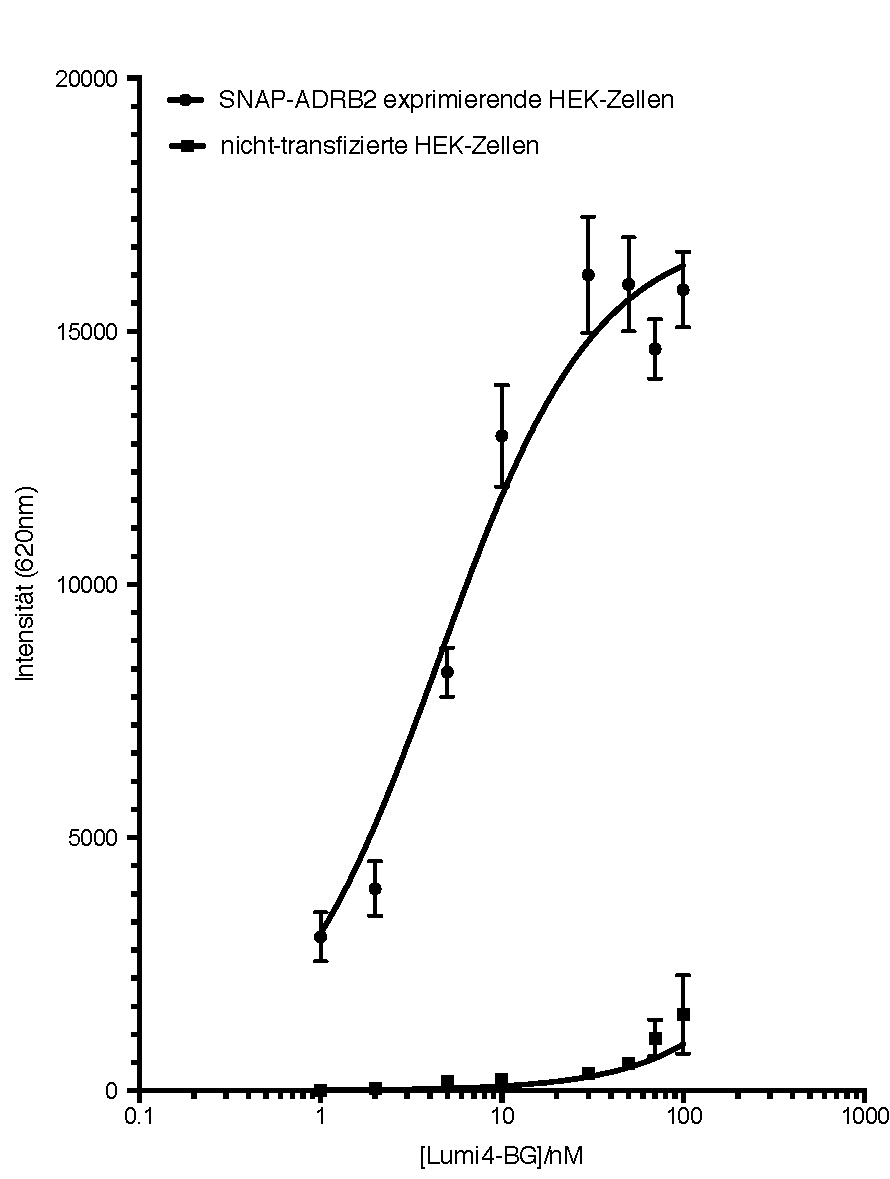
\includegraphics[width=0.6\textwidth]{lumi4binding.pdf}
    \caption{\textbf{Bindungskinetik des Lumi4-Donorfluorophors}}
    \label{fig:lumi4binding}
\end{figure}
Über steigenden Konzentrationen des SNAP-Substrates zeigte sich ein sigmoider Intensitätsverlauf, der bei spezifischer sättigbarer Bindung zu erwarten ist. Die unspezifische Bindung erwies sich als gering. Für die weitere Analyse waren mehrere Bedingungen zu optimieren: Zum einen sollte die Konzentration der SNAP-Substrate gering gehalten werden, um nicht-spezifische Bindung vernachlässigen zu können. Zum anderen war für eine zufriedenstellende signal-to-noise-ratio eine ausreichend hohe Konzentration zu wählen.

Diese Bedingung waren am besten bei der etwa halbmaximal sättigenden Konzentration des SNAP-Substrates gegeben. Für die Analyse der spezifischen Interaktion der SNAP-getaggten Rezeptoren wurde daher die Konzentration des Donor-Substrates auf 10\si{\nano M} festgelegt.

\subsubsection{Räumliche Interaktion des SNAP-getaggten \gls{beta2}}
\begin{figure}[htbp]
	\centering
    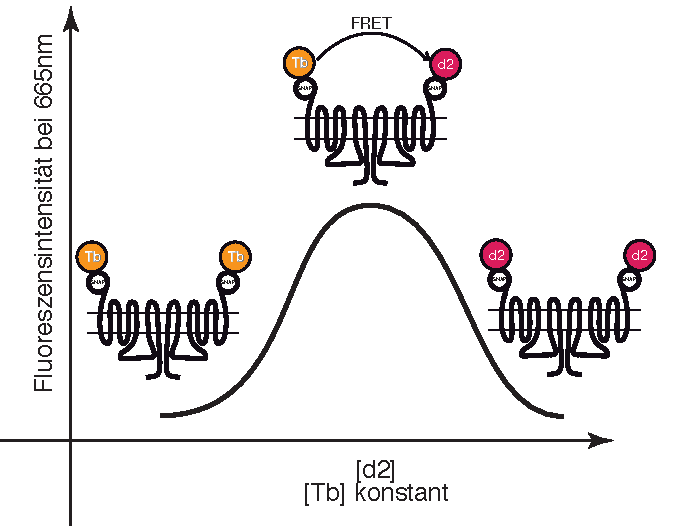
\includegraphics[width=0.5\textwidth]{bell.pdf}
    \caption{\textbf{Maximierung des FRET-Signals}}
    \label{fig:bell}
\end{figure}
    
\subsubsection{Nachweis der spezifischen Interaktion zwischen Rezeptoroligomeren}

\subsection{Einfluss der Stimulation mit Liganden des \gls{beta2} auf seine Oligomerisierung}

\subsection{Einfluss der Glycosylierung auf die Oligomerisierung des \gls{beta2}}

\section{\gls{trfret} mit fluoreszierenden Liganden des \gls{beta2}}
\label{ligandenfret}


\chapter{Diskussion}\label{chapter:diskussion}

\section{Untersuchung der Rezeptoroligomerisierung des ADRB2}
In der Vergangenheit sind auf \gls{bret} und \gls{fret} basierende Methoden zur Untersuchung der Rezeptoroligomere in Zellmembranen verwendet worden (s. Abschnitt \ref{ret}). Aufgrund hoher Komplexität und relativ geringer Signalausbeute eignen sich diese Methoden jedoch nur bedingt zur systematischen Analyse. Insbesondere weil bei den genannten Methoden häufig Membranpräparationen oder permeabilisierte Zellen verwendet werden müssen, ist die Herkunft des Signals nur schwer tatsächlich auf Rezeptoren in der Zellmembran zurückzuführen.

Demgegenüber bietet die tr-FRET-Methode mit SNAP-getaggten Rezeptoren eine deutlich höhere Signalausbeute bei klar definierter Position der räumlichen Interaktion auf die Zellmembran. Darüber hinaus findet die tatsächliche Analyse anders als in vielen älteren Assays, die die Rezeptoroligomerstruktur untersuchten, an lebenden Zellen statt. Dies bietet entscheidende Vorteile: So können beispielsweise direkt Modulatoren des Oligomerisierungsverhaltens beobachtet werden. Die Methode bietet insbesondere Vorteile bei der Untersuchung des "`Crosstalk"' zwischen heterooligomerisierten Rezeptoren. 
%TODO: tr-FRET-Möglichkeiten

\section{Möglichkeiten und Grenzen von tr-FRET zur Analyse von Rezeptoroligomerisierung}
\label{discussion:limits}

\subsection{Etablierung der tr-FRET-Methode zwischen SNAP-getaggten Rezeptoren}
Der SNAP-tag ermöglicht komfortables spezifisches Proteinlabeling. Mit 19,4\si{\kilo Da} ist er etwas kleiner als die meisten autofluoreszierenden Proteine (sie besitzen Molekulargewichte von etwa 25\si{\kilo Da}). Es gelang, ein Fusionsprotein aus ADRB2 und SNAP-tag zu klonieren. Mit dem N-terminalen tag gelang es, zuverlässig und mit hoher Spezifität ausschließlich die in der Zellmembran liegenden ADRB2 mit fluoreszierenden Molekülen zu versehen. Im Vergleich mit autofluoreszierenden Proteinen ergeben sich mit dem vorliegenden Ansatz mehrere Vorteile: Statt wenigen verfügbaren autofluoreszierenden Proteinen können mit dem Proteinlabelingsystem beliebige, insbesondere synthetische Fluorophore mit deutlich günstigeren spektralen Eigenschaften, weniger Bleicheffekten und besserer Energieeffizienz (\textit{quantum-yield}) an den zu untersuchenden Rezeptor gekoppelt werden. Außerdem ist bei einigen autofluoreszierenden Proteinen die Tendenz zur Oligomerisierung beobachtet worden, die es unbedingt auszuschließen gilt \parencite{Zhang2002a, Keppler2004}.

\subsubsection{Membranintegration des SNAP-getaggten ADRB2}
Anfangs konnte mit dem bloßen SNAP-tag am N-Terminus des ADRB2 keine Membranfärbung realisiert werden (s. Abb. \ref{fig:stainsnap}). Dabei darf nicht vergessen werden, dass es sich beim SNAP-tag um eine Protein der Größe von 20\si{\kilo Da} handelt und Einflüsse auf die korrekte Proteinadressierung denkbar sind. Insertion in die Membran war folglich erst mit einer Membraninsertionssequenz zu bewerkstelligen. Der verwendete Proteinrest ist dem murinen Htr3a-(Serotonin)-Rezeptor entnommen. Die ersten 72 Basenpaare dessen Sequenz genügen den Angaben des den SNAP-tag vermarktenden Herstellers New England Biolabs GmbH (Frankfurt a. M.) empirisch, um den mit dem SNAP-tag versehenen ADRB2 in die Zellmembran lokalisieren zu können. Damit ist gleichzeitig eine Limitation der Methode beschrieben. Zwar ist nicht davon auszugehen, dass eine N-terminale Modifikation entscheidenden Einfluss auf die Funktion des ADRB2 nimmt, doch ist bei jedem Experiment naturgemäß die geringste Komplexität zu bevorzugen. Der Versuch, auf die Membraninsertionssequenz zu verzichten und den SNAP-tag in den zweiten extrazellulären Loop zu klonieren, schlug fehl. Da es Hinweise gibt, dass die extrazellulären Loops außerdem als Interface der Dimerisierung fungieren könnten \parencite{Salahpour2004}, ergab sich außerdem der sinnvollere Kompromiss zu dem N-terminal lokalisierten SNAP-tag.

\subsubsection{Kandidaten für eine Beeinflussung der Rezeptoroligomerisierung}
Im gleichen Zusammenhang sollte eine \textit{dimerisierungsdefiziente} Mutation des ADRB2 untersucht werden. In einer Publikation von Salahpour et al. (2004) war mit einem BRET-basierten Assay die Dimerisierung als Voraussetzung für die Adressierung des ADRB2 in die Zellmembran gefunden worden. Interessanterweise deckt sich die Lokalisation mit der beim CXCR4-Chemokin-Rezeptor in der Kristallstruktur gefundenen Transmembrandomäne als Dimerisierungsinterface \parencite{Wu2010}. Die Daten bezüglich des ADRB2 finden sich jedoch danach nicht mehr erneut durch andere Gruppen verifiziert. In der Versuchsreihe der vorliegenden Arbeit gelang mit der beschriebenen Mutation Tyr284 in der sechsten Transmembrandomäne des ADRB2 keine Expression des Rezeptors. Nicht ausgeschlossen ist die Vermutung, dass die Oligomerisierung tatsächlich Voraussetzung für die korrekte Membraninsertion sein könnte.

Auch ein in einer anderen Arbeit \parencite{Hebert1996} publiziertes Peptid der sechsten Transmembrandomäne (\textit{TM VI}) fand in Publikationen weiter keine Beachtung und war insofern nicht überzeugend in den vorliegenden Aufbau zu integrieren, als mit einfacher Zugabe eines Peptids nicht von seiner Integration in die Zellmembran auszugehen ist. 

\subsubsection{SNAP- und CLIP-basierte Membranfärbungen}
Für die Färbung mithilfe des SNAP-tags erwiesen sich die mit Alexa-488 versehenen SNAP-Substrate als geeignete Fluorophore (dargestellt in Abbildung \ref{snapmikro}). In der Fluoreszenzmikroskopie konnten kontrastreiche Bilder mit geringer Hintergrundfluoreszenz und vernachlässigbarem unspezifischem Signal aufgenommen werden. Die Kreuzreaktivität der SNAP-Substrate mit der enzymatischen Aktivität des CLIP-tags konnte ausgeschlossen werden. Eine mit dem CLIP-tag versehene Variante des ADRB2 wurde kloniert - fand aber, da es bei den vorliegenden Versuchsreihen primär um den Nachweis von Homooligomeren ging, vorerst keine Anwendung. Für spätere Untersuchungen, die sich an Heterooligomere richten, kommt dem orthogonal zum SNAP-tag gleichzeitig nutzbaren CLIP-tag große Bedeutung zu.


\subsection{Hinreichende Kriterien zum Nachweis der Rezeptoroligomerisierung}
Tr-FRET-basierte Studien bieten Sensitivität, die auch für den Nachweis von Rezeptoroligomeren auf nativen Gewebsstücken ausreichend sein kann \parencite{Albizu2010}. Streng genommen kann die Rezeptoroligomerisierung mit der vorliegenden Methode im Prinzip nicht direkt beobachtet werden. Es galt also, um die Messergebnisse überzeugend als auf oligomerisierten SNAP-getaggten Rezeptoren beruhend zu interpretieren mehrerer Versuchsreihen:

Zuerst war, wie im vorigen Abschnitt diskutiert, die korrekte Lokalisation des Fusionsproteins nachzuweisen. Diese war mit mikroskopischer Methoden gelungen und notwendig, weil alle weiteren Untersuchungen readerbasiert durchgeführt wurden und der Reader stets nur die Gesamtintensität eines Wells messen konnte - ungeachtet der subzellulären Lokalisation (s. Abschnitt \ref{reader}). Dabei war unspezifische Hintergrundfluoreszenz durch die beschriebenen intrinsischen Vorteile der genutzten Fluorophore und der tr-FRET-Methode per se limitiert. Weiter konnte durch das zügige Readout multipler Wells jeweils einer Bedingung statistische Signifikanz schnell identifiziert und Messfehler minimiert werden. 

Bei jedem Experiment, das die räumliche Nähe von Proteinen untersucht, ist auszuschließen, dass es sich nicht lediglich um der Rezeptordichte geschuldete und somit direkt von der Expressionsstärke abhängige Interaktion handelt. Im vorliegenden Fall war dazu die im Ergebnisteil erläuterte Methode verwendet worden. Erst mit der Beobachtung, dass die tr-FRET-Intensität direkt den exprimierten Rezeptoren proportional war - und nicht etwa in exponentiellem Zusammenhang stand - konnte die Kollisionshypothese verworfen werden.



\subsection{Modulation der Oligomergröße und Rezeptorkonformationsänderungen durch Ligandenstimulation}
\label{dis:stimulation}
In Abschnitt \ref{res:stimulation} konnte beobachtet werden, dass Stimulation mit Agonisten einen signifikanten Effekt auf die tr-FRET-Ratio der SNAP-getaggten Rezeptoren nimmt. Die Steigerung des tr-FRET-Signals wurde insbesondere bei langer Stimulation sichtbar und war nicht bei Vorbehandlung mit inversen Agonisten oder Antagonisten zu beobachten.

Nun sind unabhängig von den Ergebnissen anderer Untersuchungen eine Reihe von Möglichkeiten zu diskutieren, die in einer derartigen Erhöhung des FRET-Signals resultieren könnten. 

\subsubsection{De-novo-Formation von Rezeptorligomeren}
Es ist denkbar, dass durch die Behandlung mit Agonisten des ADRB2 neue Rezeptoroligomere aus zuvor monomeren Rezeptoreinheiten rekrutiert werden. Geht man davon aus, dass diese neu geformten Oligomere von der gleichen Größe wie die ursprünglichen waren, ergibt sich ein zusätzliches tr-FRET-Signal (bei 665\si{\nano\meter}) bei gleichzeitig verringertem Donor-Signal (bei 620\si{\nano\meter}); das am neu geformten Oligomer beteiligte Donorfluorophor verliert den größten Teil seiner Strahlungsintensität an die Förster-Interaktion mit dem Akzeptor). In den Ergebnissen wurde stets die Ratio, also der Quotient aus Akzeptor- und Donorintensität gemessen. Wenn man nun bedenkt, dass auch die nicht-oligomerisierten Rezeptorprotomere mit jeweils geringeren Beträgen der Akzeptor- und höheren der Beträgen Donorwellenlänge in die ursprüngliche tr-FRET-Ratio eingegangen waren, ergibt sich in der Summe eine Erhöhung der tr-FRET-Ratio bei Neubildung eines Oligomers aus primär nicht oligomerisierten Rezeptoren. Neubildung von Rezeptoroligomeren würde sich mit der vorliegenden Methode als größere tr-FRET-Ratio äußern bzw. kann als Ursache einer gegenüber der Ausgangssituation gestiegenen tr-FRET-Ratio nicht ausgeschlossen werden.

\subsubsection{Änderung der Anzahl der Protomere in einem Rezeptoroligomer}
Ebenso für die Signaländerung verantwortlich könnte neben der de-novo-Formation von Rezeptoroligomeren auch eine Änderung der Anzahl der an einem Rezeptoroligomer beteiligten Rezeptoren verantwortlich sein. Analog zu obiger Kalkulation würde, wenn zuvor monomere Rezeptoren zu einem Rezeptoroligomer hinzukommen, eine erhöhte tr-FRET-Ratio resultieren. Ein bloßer Zusammenschluss von bereits zuvor oligomerisierten, am tr-FRET-Signal beteiligten Rezeptoren, würde demgegenüber nicht zu veränderter tr-FRET-Ratio beitragen.

Verfügt man nur über die tr-FRET-Ratio an einem Messpunkt mit festgesetzter Donor- und Akzeptorkonzentration, können keine Aussagen über die Anzahl der Rezeptoren in einem Oligomer getroffen werden. Insofern ist auch die Änderung dieser Anzahl bei Stimulation a priori nicht als Ursache des größeren Signals auszuschließen. An dieser Stelle wurde daher erneut das Experiment durchgeführt, bei dem die Akzeptorkonzentration gegenüber fester Donorkonzentration variiert wird. Wie bereits in \ref{res:stimulation} geschildert, würde sich bei zunehmender Oligomergröße eine breitere Gauß-Verteilung des Signals ergeben. Da aber die erhaltene Gauß-Verteilung in direkter proportionaler Beziehung zur ursprünglichen stand, d.h. die neue Gauß-Verteilung sich durch Multiplikation mit einem für alle Funktionswerte konstanten Faktor aus der alten transformieren ließ, kann nicht davon ausgegangen werden, dass sich die Größe der Oligomere mit Ligandenstimulation geändert hatte.

\subsubsection{Rezeptorkonformationsänderungen}
Das tr-FRET-Signal ist für einen effizienten Energietransfer von einer optimalen Entfernung zwischen den interagierenden Fluorophoren abhängig. Der optimale Energietransfer findet bei einem festen Radius statt. Bei dem definierten Radius $R_0$ (Förster-Radius) beläuft sich die Effizienz des Energietransfers konstitutiv auf 50\%. Variation der Entfernung zwischen Donor- und Akzeptorfluorophoren um einen Betrag $\Delta R$ führt demnach zu einer neuen FRET-Effizienz $E=R_0^6/(\Delta R^6+R_0^6)$. Dabei befindet sich $R_0$ für Fluorophore wie die hier verwendeten üblicherweise im Bereich von $46 \times 10^{-10}$\si{\meter} \parencite{Doumazane2011, Maurel2008}. Es ergibt sich, dass eine Änderung der Entfernung der FRET-Partner einen signalerhöhenden Effekt auf die tr-FRET-Ratio haben kann. Somit ist denkbar, dass bereits minimale Rezeptorkonformationsänderungen mit messbarer Änderung des tr-FRET-Signals einhergehen kann.

Bei Untersuchungen der Kristallstruktur des ADRB2 wurde dem unstrukturierten N-Terminus insbesondere bei der Ligandenbindung Bedeutung beigemessen \parencite{Cherezov2007}. Im vorliegenden Aufbau war der SNAP-tag N-terminal an das Fusionsprotein kloniert worden. 


\begin{figure}[htbp]
	\centering
    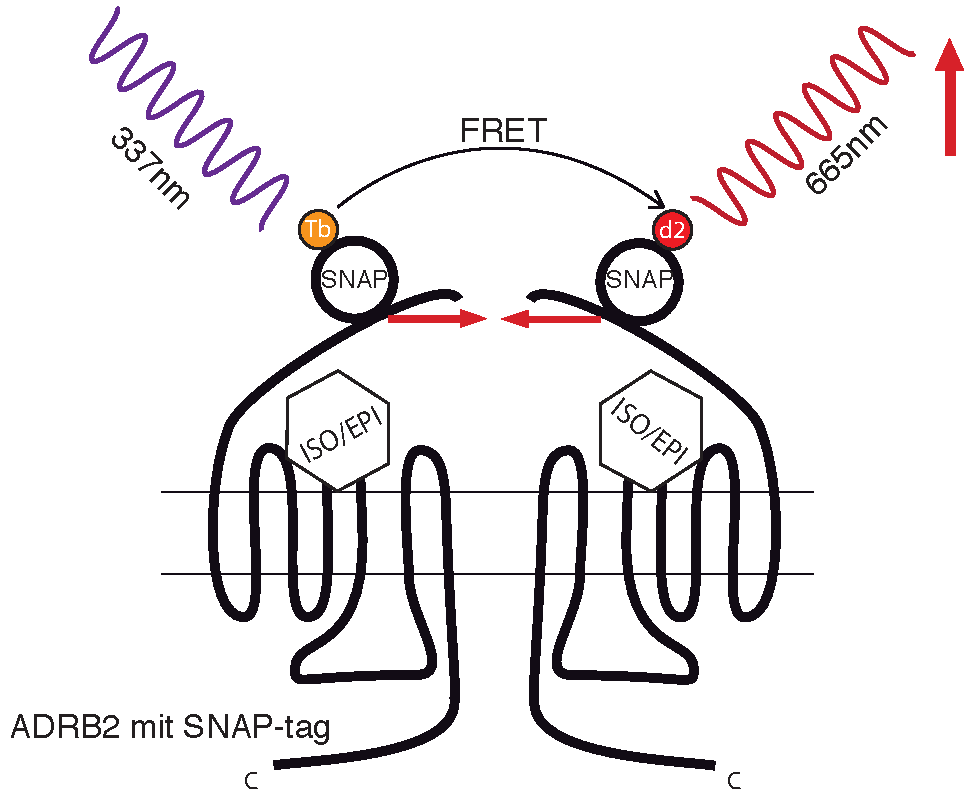
\includegraphics[width=0.6\textwidth]{fig_stimmov.pdf}
    \caption{\textbf{N-terminale Veränderung bei Stimulation des ADRB2 mit Agonisten:} In einem denkbaren Szenario bewirken agonistische Liganden eine Bewegung des N-Terminus des ADRB2 und führen so zu höherer tr-FRET-Intensität.} 
    \label{fig:stimmov}
\end{figure}

Führt nun die Bindung von Agonisten - im Gegensatz zu der Bindung von Antagonisten - zu Konformationsänderungen des N-Terminus wie in Abbildung \ref{fig:stimmov} illustriert, resultiert ein möglicherweise optimierter Abstand zwischen den tr-FRET-Partnern und damit ein höheres tr-FRET-Signal. Andere Studien, die auch intramolekulare FRET-Effekte - und damit rezeptorinterne Konformationsänderugen in Betracht zogen, attribuierten Agonisteneffekte den Konformationsänderungen in Transmembrandomäne VI (TM VI) \parencite{Fung2009, Latif2002, Zhu2002}.

Die agonistabhängigen tr-FRET-Änderungen sind also gut mit Rezeptorkonformationsänderungen erklärbar. Mit dem Ansatz lässt sich nicht bestimmen, an welcher Stelle des Rezeptors die entscheidenden Konformationsänderungen stattfinden würden. 

\subsubsection{Rezeptorinternalisierung}
In Abbildung \ref{fig:internalization} konnten morphologische Anhaltspunkte der Rezeptorinternalisierung bei Stimulation mit Agonisten gefunden werden. Dabei war das primär zellimpermeable Fluorophor Alexa Fluor 488 nach kovalenter Bindung an den SNAP-tag unter Stimulation innerhalb der Zellmembran zu sehen. Ursprünglich sollte die Oligomerisierung des ADRB2 an der Zellmembran untersucht werden. Die mögliche Internalisierung des ADRB2 stellt dabei eine Situation dar, unter der das tr-FRET-Signal nicht mehr eindeutig verwertbar ist. 

Bereits kurze Stimulation mit Agonisten unter Kulturbedingungen führt im Falle des ADRB2 zu Endozytose und Rezeptorinternalisierung aus der Zellmembran \parencite{VonZastrow1994}. N-terminal SNAP-getaggte Rezeptoren sind in neueren Publikationen zur Untersuchung von Rezeptorinternalisierung verwendet worden \parencite{Roed2014}. In der Publikation von Roed et al. (2014) diente der ADRB2 als Referenz für Rezeptorinternalisierung. Bereits nach zehnminütiger Stimulation mit Isoproterenol bei der Konzentration 1\si{\nano M} konnte tr-FRET-basiert die Internalisierung eines Großteils der Rezeptoren beobachtet werden.

In einer BRET-basierten Studie war geschlossen worden, dass Rezeptorinternalisierung des ADRB2 zur Dissoziation der Rezeptoroligomere führte \parencite{Lan2011}. Davon ist mit den hier gewonnenen Daten nicht auszugehen. Im Gegenteil suggeriert das angehobene tr-FRET-Signal eher einen dichteren Rezeptorverband.

Zusammenfassend ist eine Signalanhebung bei Ligandenstimulation wie unter den hier beschriebenen Bedingungen ist gut mit der dichteren Agglomeration von Rezeptoren vereinbar, wie sie unter endozytotischen Bedingungen zu erwarten ist.  

\subsubsection{Interpretation}
In der Literatur wird über eine mögliche Rolle der Assoziation bzw. Dissoziation von Oligomeren bei Stimulation mit Liganden berichtet. In einigen Publikationen führte Stimulation mit Liganden zu postulierter Assoziation \parencite{Angers2000} andere berichten über keine Änderung der Anzahl der an einem Oligomer beteiligten Protomere \parencite{Dorsch2009}. In weiteren Publikationen wird die konformationelle Änderung der Protomere gegenüber den angrenzenden (intermolekulares FRET) als Ursache agonistenbedingter Signaländerung angeführt \parencite{Fung2009}. Die Anzahl der in einem Oligomer befindlichen Protomere scheint von Rezeptor zu Rezeptor unterschiedlich zu sein. FRAP-basiert gemessen ergaben sich für den ADRB2 Hinweise auf höhergradige Oligomere \parencite{Dorsch2009}. Eine neuere Publikation, die sich aufwendiger FCS- und PCH-Untersuchungen bedient \parencite{Herrick-Davis2013}, kommt zum Schluss, dass es sich unter anderem im Fall des ADRB2 um strikte Dimere handelt und höhergradige Oligomere wiederum nicht vorkommen. Die hier gefundenen Ergebnisse widersprechen diesen nicht, liefern jedoch - der Eigenschaften der tr-FRET-Methode geschuldet - per se keine eindeutige Gradierung der Oligomere. 

Die mit der vorliegenden Methode gewonnenen Ergebnisse sind sowohl mit Rezeptorkonformationsänderungen als auch mit Effekten der Rezeptorinternalisierung vereinbar. Der beobachtete Effekt war bei längerer Stimulation von größerem Betrag. Ebenso verhielten sich die morphologisch festgehaltenen Veränderungen der Rezeptorlokalisation. Es existiert also eine positive Korrelation zwischen Rezeptorinternalisierung und vergrößerter tr-FRET-Ratio. Ohne weitere Untersuchung - beispielsweise mit Inhibition der Rezeptorinternalisierung - ist diese nicht als Ursache der Änderung beweisen, erscheint jedoch auch in Kombination mit Konformationsänderungen als plausible Möglichkeit. 

Ebenso wahrscheinlich erscheinen Konformationsänderungen innerhalb des Rezeptors oder im räumlichen Verhalten der Protomere zueinander. 

Assoziations- oder Dissoziationseffekte von Protomeren konnten als Ursache des veränderten tr-FRET-Signals ausgeschlossen werden. 

\subsection{Anwendung auf tr-FRET zwischen Rezeptorliganden}


\subsubsection{tr-FRET zwischen fluoreszierenden Liganden des ADRB2 in HEK293-Zellen}

Mit den vorliegenden Ergebnissen ist es gelungen, Rezeptoroligomere des nicht-modifizierten \gls{beta2} nachzuweisen. Dabei wurden tr-FRET-geeignete Liganden synthetisiert. 

Aufgrund der möglichen funktionellen Interaktion mit den zu untersuchenden Rezeptoren, die in Abschnitt \ref{res:stimulation} festgestellt worden war und Beobachtungen in der Literatur, nach denen mit Agonisten teils geringere Signalausbeute erreicht wurde \parencite{Albizu2010, Emami-Nemini2013}, erfolgte die de-novo Synthese eines in Bezug auf Rezeptorinternalisierung und Affinitätsänderung durch Phosphorylierungseffekte inerten Ligandenderivats. Der inverse Agonist ICI-118,551 besitzt äußerst hohe Affinität und Spezifität für den \gls{beta2} ($K_D=4.6 \pm 2\si{\nano M}$) \parencite{Mauriege1988}. Dem Labor von Prof. Dr. Peter Gmeiner (Universität Erlangen) war die Synthese eines funktionellen Liganden mit einem Linker und den daran gekoppelten Fluorophoren Lumi4 und Alexa647 gelungen. Erst mit dieser Verbindung waren Experimente möglich.

Zum Nachweis der Spezifität des FRET-Signals für die Rezeptoroligomere wurden mehrere Experimente durchgeführt: Es konnte im Assay zur Analyse der spezifischen Bindung des Ligandenderivats eine typische Affinitätskurve gemessen werden (s. Abb. \ref{fig:ligandsat}). Damit war die Funktionalität des Liganden gezeigt. Die beiden Ligandenspezies (tr-FRET-Donor- und Akzeptorliganden) zeigten in einem Kompetitionsassay den für Rezeptoroligomere typischen gauß-verteilten Intensitätsverlauf des tr-FRET-Signals (s. Abb. \ref{fig:ligandoncells}. So konnte die für tr-FRET notwendige räumliche Nähe der Rezeptoren gezeigt werden. In Kompetition mit nicht-getaggten Liganden war das tr-FRET-Signal vollständig eliminierbar. Dies deutet abermals auf den spezifischen rezeptorgebundenen Ursprung des Signals hin. 

In der Zusammenschau mit den Ergebnissen aus den SNAP-tag-gestützten Untersuchungen konnte die Hypothese verworfen werden, dass das tr-FRET-Signal lediglich der Kollision monomerer Rezeptoren geschuldet war (s. Abb. \ref{fig:correlation}).

Analog zu den Ergebnissen, die bei SNAP-getaggten Rezeptoren gewonnen werden konnten, stellt sich die Frage nach dem Verhalten der nicht-modifizierten Rezeptoren unter Stimulation. Da aber die Ligandenbindungsstelle durch die fluoreszierenden Liganden bereits zumindest zum Teil für Agonisten nicht mehr zugänglich ist und die Rezeptoreigenschaften durch die Interaktion mit dem inversen Agonisten ICI-118,551 verändert sind, bestand diese Möglichkeit in der vorliegenden Versuchsreihe nicht mehr.

\subsubsection{Untersuchungen des nativ exprimierten ADRB2}

Für zukünftige Experimente mit dem nativ exprimierten ADRB2 etwa bei der Analyse von Gewebsstücken kann folgendes geschlossen werden: Unter nativen Umständen ist mit deutlich geringerer Expression (s.u.) zu rechnen als im Falle eines Überexpressionssystems. Die Kollisionshypothese konnte aber schon unter Bedingungen der Überexpression der SNAP-getaggten Rezeptoren ausgeschlossen werden. Somit erscheint für den ADRB2 die zufällige Kollision als Ursache für das gemessene tr-FRET-Signal als unwahrscheinlich.

In anderen Versuchsreihen war unter sonst gleichen Bedingungen mit Rezeptoragonisten ein geringeres tr-FRET-Signal als mit -antagonisten beobachtet worden. Der Effekt ist auf das negativ-kooperative Bindungsverhalten von Agonisten im Vergleich zu den Antagonisten zurückgeführt worden und liefert weitere Evidenz für die Existenz von Rezeptoroligomeren im Gegensatz zur Kollisionshypothese \parencite{Cottet2012a}. Träfe die Kollisionshypothese zu, sollten mit Rezeptorantagonisten und -agonisten Signale gleicher Größenordnung zu beobachten sein. Gleichzeitig wird eine prinzipielle Limitation bei dem alleinigen Einsatz der ligandenbasierten Methode ersichtlich: Der Einsatz von Liganden selbst hat möglicherweise Einfluss auf die Oligomerisierung. Flankiert man solche Studien mit Fusionsproteinen aus dem Rezeptor und einem Proteinlabelingsystem wie in der vorliegenden Arbeit, können über den Einfluss der Liganden erst Aussagen getroffen werden.

\subsubsection{Die Rezeptoren der Lungenepithelzelllinien Calu-3, 16HBEo14 und A549 können mit der tr-FRET-Methode nicht auf ihre Oligomerisierungseigenschaften überprüft werden}
Von weiterer Bedeutung ist die in-vivo-Analyse der Oligomerisierung des \gls{beta2}. Dazu wurden drei Lungenepithelzelllinien (LEC) untersucht, die endogen über ein hohes Expressionsniveau verfügen sollen \parencite{Abraham2004}. Sowohl bei den Calu-3-, als auch bei 16HBEo14- und A549-Zellen konnte aber in Versuchsreihen analog zu den mit \gls{beta2} transfizierten HEK293-Zellen keine ausreichend hohe Signalausbeute erreicht werden. So war zum einen keine Gauß-Verteilung  bei Variation des Akzeptorliganden messbar (s. Abb. \ref{fig:ligandoncells}) und zum anderen auch unter Zugabe einer hohen Konzentration unmarkierten Ligands keine Reversibilität des tr-FRET-Signals zu messen (s. Abb. \ref{fig:iciexcess}). Es ist daher davon auszugehen, dass selbst mit dem hochaffinen fluoreszierenden Liganden keine ausreichende Sensitivität für das Expressionsniveau der Lungenepithelzellen erreicht werden konnte. 

Welchen Grenzwert die Methode tatsächlich aufweist, ist schwer zu bewerten. In der Literatur ist mit ähnlichen Assays der Nachweis nativer Rezeptoren bei einer Expressionsstärke von etwa $1-3 \si{\pico \mol / \milli\gram}$ Protein gelungen \parencite{Albizu2010}. Demgegenüber ist die Rezeptordichte bei den verwendeten Lungenepithelzellen mit nach Radioligandenbindung gemessenen 10000 Rezeptoren pro Zelle um etwa das 30-fache geringer \parencite{Abraham2004}. Die Detektionsschwelle für fluoreszierende Liganden bei der vergleichbaren Methode der Fluoreszenzpolarisation liegt ebenfalls bei etwa $1 \si{\pico \mol / \milli\gram}$ Protein \parencite{Gagne2002, DeJong2005}. 

\section{Ausblick}
\subsubsection{Nutzung von tr-FRET-getaggten Liganden in der Arzneimittelforschung}
Mit ligandengebundenen tr-FRET-Fluorophoren können im Hochdurchsatzverfahren neue Verbindungen auf ihre Eigenschaften an Rezeptoren getestet werden. Im Vergleich zu anderen Methoden wie beispielsweise der Radioligandenbindung bieten Untersuchungen mit tr-FRET-Liganden den Vorteil des komfortablen und sicheren Umgangs. Experimente können, wie in den Versuchen in dieser Arbeit, problemlos im 96- und 384-well-Format durchgeführt werden. Das Readout verläuft automatisiert mit tr-FRET-kompatiblen Readern wie dem hier verwendeten (s. Abschnitt \ref{material}).


\chapter{Zusammenfassung}\label{chapter:zusammenfassung}


\appendix{}


\microtypesetup{protrusion=false}
\listoffigures{}
\listoftables{}
\microtypesetup{protrusion=true}
\printbibliography{}

\end{document}